\documentclass{ieeeojies}
\usepackage{cite}
\usepackage{amsmath,amssymb,amsfonts}
\usepackage{algorithmic}
\usepackage{graphicx}
\usepackage{textcomp}
\usepackage{array}
\usepackage[table]{xcolor}
\usepackage{multirow}
\usepackage{multicol}
\usepackage{float}
\usepackage{amsmath}
\usepackage{algorithm}

\def\BibTeX{{\rm B\kern-.05em{\sc i\kern-.025em b}\kern-.08em
    T\kern-.1667em\lower.7ex\hbox{E}\kern-.125emX}}

\begin{document}
\raggedbottom
\title{Leveraging Statistical and Machine Learning models to forecast stock prices of Vietnamese tech companies}

\author{\uppercase{Ninh Thien Bao}\authorrefmark{1},
    \uppercase{Dao Tien Dat\authorrefmark{2}, and Dao Minh Huy}\authorrefmark{3}}

\address[1]{Faculty of Information Systems, University of Information Technology, (e-mail: 21520621@gm.uit.edu.vn)}
\address[2]{Faculty of Information Systems, University of Information Technology, (e-mail: 21521930@gm.uit.edu.vn)}
\address[3]{Faculty of Information Systems, University of Information Technology, (e-mail: 21520912@gm.uit.edu.vn)}

\markboth
{Author \headeretal: Ninh Thien Bao, Dao Tien Dat, Dao Minh Huy}
{Author \headeretal: Ninh Thien Bao, Dao Tien Dat, Dao Minh Huy}

\begin{abstract}
    Predicting stock prices of Vietnamese tech companies presents a unique challenge due to the dynamic and rapidly evolving nature of the technology sector in Vietnam. This study focuses on investigating the efficacy of statistical models and machine learning algorithms in forecasting stock prices of prominent tech firms. Leveraging historical stock market data specific to the tech sector in Vietnam, an extensive analysis of various predictive models is conducted, including SARIMAX, Gradient Boosting Regressor, Dlinear, Linear Regression, ARIMA, as well as recurrent neural network (RNN) architectures such as Gated Recurrent Units (GRU) and Long Short-Term Memory (LSTM) networks. The investigation evaluates the performance of each algorithm in terms of prediction accuracy, robustness, and computational efficiency, with a focus on predicting stock prices of key players in the Vietnamese tech industry, including FPT Corporation (FPT), Innovative Technology Development Corporation (ITD) and CMC Corporation (CMG). Additionally, the insights derived from this study contribute to advancing the understanding of effective methodologies for predicting stock prices of Vietnamese tech companies, providing valuable guidance for investors, financial analysts operating in this dynamic sector.
\end{abstract}

\begin{keywords}
    Forecast stock price, Linear regression, Gated Recurrent Units, GRU, Long Short-Term Memory, LSTM, Recurrent Neural Network, RNN, ARIMA, SARIMAX, Gradient Boosting Regressor, GBR, Decomposition Linear, Dlinear
\end{keywords}

\titlepgskip=-15pt

\maketitle

\section{Introduction}
\label{sec:introduction}
The stock market plays a pivotal role in the global economy, serving as a platform for companies to raise capital and for investors to allocate funds with the expectation of returns. In Vietnam, as in many emerging economies, the stock market is characterized by unique dynamics influenced by factors such as economic development, regulatory environment, and investor sentiment. Accurately predicting stock prices in such markets is essential for investors, financial analysts, and policymakers alike as it enables informed decision-making, risk management, and the efficient allocation of resources.

However, forecasting stock prices is a highly challenging task due to the complexity and volatility of financial markets. Traditional methods of analysis, such as fundamental analysis and technical analysis, often fall short in capturing the complex patterns and nonlinear relationships present in stock price movements. In the last few years, there has been a growing interest in the application of statistical models and machine learning techniques to address this challenge, driven by advances in computational power, data availability, and algorithmic sophistication.

This research aims to investigate the effectiveness of using statistical models and machine learning algorithms to predict stock prices of Vietnamese tech companies. By leveraging historical stock market data from Vietnam, we seek to evaluate the performance of various predictive models and assess their ability to capture the unique characteristics of the Vietnamese stock market. Specifically, we will explore the predictive power of regression models, time series analysis techniques, and advanced machine learning algorithms.

Furthermore, we will examine the impact of incorporating different types of features, including financial indicators, market sentiment, and macroeconomic factors, on the accuracy of stock price predictions. By analyzing a diverse set of features, we aim to identify the key drivers of stock price movements in the Vietnamese market and provide insights into the factors that influence investor behavior and market dynamics.

Overall, this study contributes to the growing body of research on stock price prediction in emerging markets and provides valuable insights for investors, financial analysts operating in the Vietnamese context. By leveraging advanced analytical techniques, we aim to enhance our understanding of stock market dynamics and improve the accuracy of stock price forecasts, ultimately facilitating more informed investment decisions and promoting the efficient functioning of financial markets.
\section{Related Works}
The prediction of stock prices through the use of a combination of statistical models and machine learning techniques has received a lot of interest in recent years. Pai and Lin (2005) \cite{b1} proposed a hybrid methodology combining the autoregressive integrated moving average (ARIMA) model with support vector machines (SVMs) for stock price forecasting. Their approach aimed to harness the strengths of both models, with computational tests demonstrating promising results in capturing nonlinear patterns within stock price data.

Vijh et al. (2020) \cite{b2} explored the use of Artificial Neural Networks (ANNs) and Random Forest techniques to predict the closing prices of stocks. By utilizing financial data such as Open, High, Low, and Close prices, their models exhibited efficiency in forecasting the next day's closing price for various companies across different sectors. Evaluation metrics including Root Mean Square Error (RMSE) and Mean Absolute Percentage Error (MAPE) indicated the effectiveness of their predictive models.

Nelson, Pereira, and Oliveira (2017) \cite{b3} delved into the application of Long Short-Term Memory (LSTM) neural networks for predicting stock price movements. Their study focused on capturing the complex and dynamic nature of stock market environments by incorporating historical price data and technical analysis indicators. Through a series of experiments, they achieved promising results, with their LSTM-based model demonstrating an average accuracy of 55.9\% in predicting future trends of stock prices.

These studies collectively illustrate the diverse approaches undertaken to tackle the challenge of stock price prediction, ranging from hybrid statistical and machine learning models to advanced neural network architectures.
\section{Materials}
\subsection{Dataset}
These three datasets were gathered by using the VnStock program. These datasets are time-series dataset related to historical stock prices of Vietnamese big tech company including FPT Corporation (FPT), Innovative Technology Development Corporation (ITD) and CMC Corporation (CMG) and span from March 1, 2019 to June 1, 2024. All of the datasets include the following attribute:
\begin{itemize}
    \item Time: This field represents the time at which the stock data was recorded.
    \item Open: This field represents the opening price of the stock at the given time period. The opening price is the price at which the first trade of the day occurred.
    \item High: This field represents the highest price the stock reached during the given time period.
    \item Low: This field represents the lowest price the stock reached during the given time period.
    \item Close: This field represents the closing price of the stock at the given time period. The closing price is the price at which the last trade of the day occurred.
    \item Volume: This field represents the total volume of shares traded during the given time period. Volume typically refers to the number of shares that were traded during a specific period.
    \item Ticker: This field represents the ticker symbol or stock symbol of the company whose stock data is being recorded. Ticker symbols are unique alphabetic identifiers assigned to publicly traded companies.
\end{itemize}

\subsection{Descriptive Statistics}
\begin{table}[H]
    \centering
    \caption{Descriptive Statistics for FPT, CTR, and CMG}
    \begin{tabular}{|>{\columncolor{red!20}}c|c|c|c|}
        \hline
        \rowcolor{red!20}  & FPT           & CMG          & ITD          \\ \hline
        Count              & 1313          & 1313         & 1313         \\ \hline
        Mean               & 56880.087     & 26832.39     & 10160.89     \\ \hline
        Median             & 63470         & 28380        & 10040        \\ \hline
        Mode               & 68400         & 31300        & 7560         \\ \hline
        Standard Deviation & 27473.98      & 10097.55     & 3002.802     \\ \hline
        Standard Error     & 758.209       & 278.665      & 82.8694      \\ \hline
        Sample Variance    & 754819638.968 & 101960621.57 & 9016823.3029 \\ \hline
        Kurtosis           & -0.39622      & -0.207957    & 0.865044898  \\ \hline
        Skewness           & 0.46246       & 0.49889      & 0.923718     \\ \hline
        Range              & 118810        & 52720        & 16110        \\ \hline
        Minimum            & 19190         & 10880        & 5320         \\ \hline
        25\%               & 28410         & 17810        & 7550         \\ \hline
        75\%               & 71450         & 34350        & 11650        \\ \hline
        Maximum            & 138000        & 63600        & 21430        \\ \hline
        Sum                & 74683554      & 35230929     & 13341255     \\ \hline
    \end{tabular}
\end{table}
\begin{figure}[H]
    \centering
    \begin{minipage}{0.23\textwidth}
        \centering
        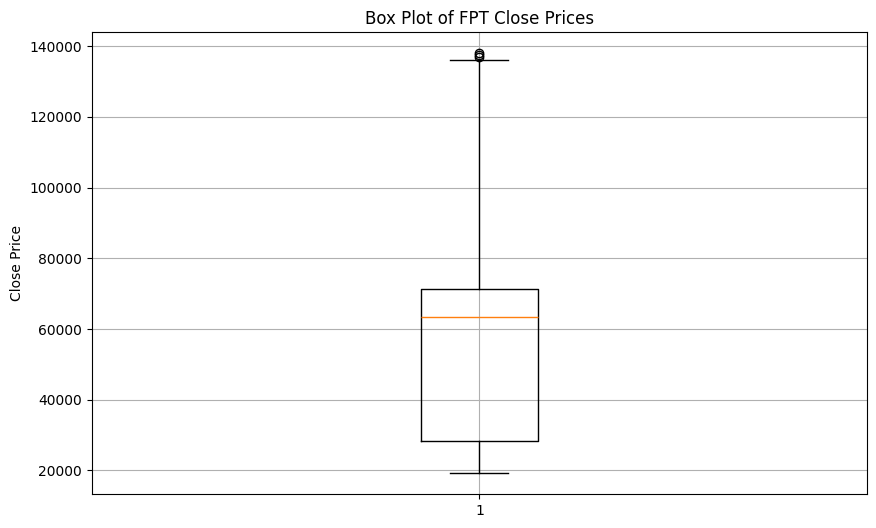
\includegraphics[width=1\textwidth]{bibliography/Figure/FPT_Boxplot.png}
        \caption{FPT stock price's boxplot}
        \label{fig:1}
    \end{minipage}
    \hfill
    \begin{minipage}{0.23\textwidth}
        \centering
        \includegraphics[width=1\textwidth]{bibliography/Figure/FPT_histogram.png}
        \caption{FPT stock price's histogram}
        \label{fig:2}
    \end{minipage}
\end{figure}
\begin{figure}[H]
    \centering
    \begin{minipage}{0.23\textwidth}
        \centering
        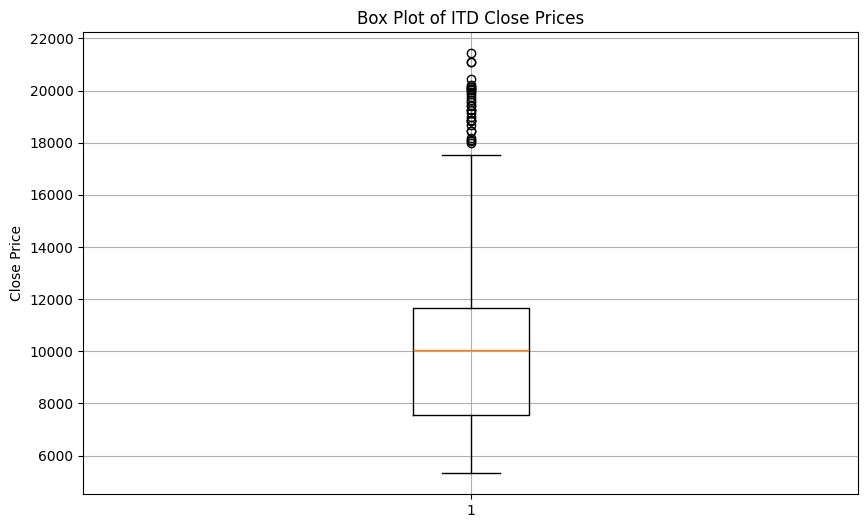
\includegraphics[width=1\textwidth]{bibliography/Figure/ITD_Boxplot.png}
        \caption{ITD stock price's boxplot}
        \label{fig:1}
    \end{minipage}
    \hfill
    \begin{minipage}{0.23\textwidth}
        \centering
        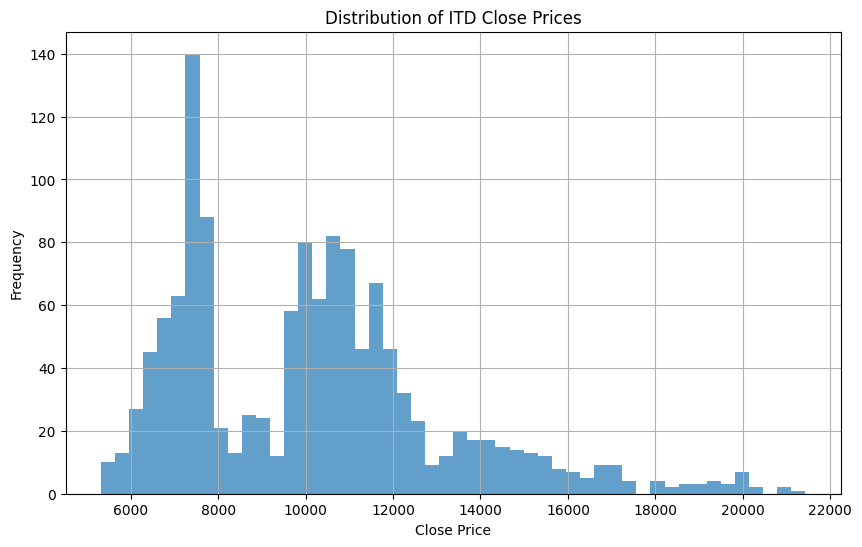
\includegraphics[width=1\textwidth]{bibliography/Figure/ITD_histogram.png}
        \caption{ITD stock price's histogram}
        \label{fig:2}
    \end{minipage}
\end{figure}

\begin{figure}[H]
    \centering
    \begin{minipage}{0.23\textwidth}
        \centering
        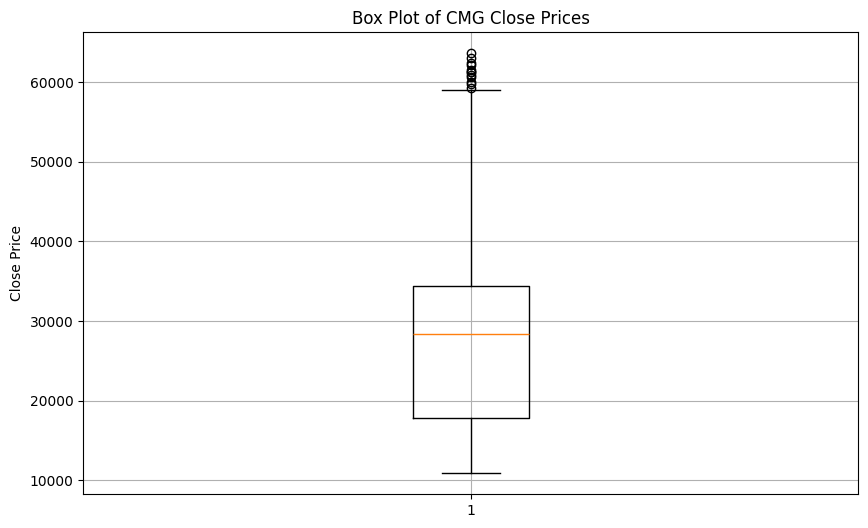
\includegraphics[width=1\textwidth]{bibliography/Figure/CMG_Boxplot.png}
        \caption{CMG stock price's boxplot}
        \label{fig:1}
    \end{minipage}
    \hfill
    \begin{minipage}{0.23\textwidth}
        \centering
        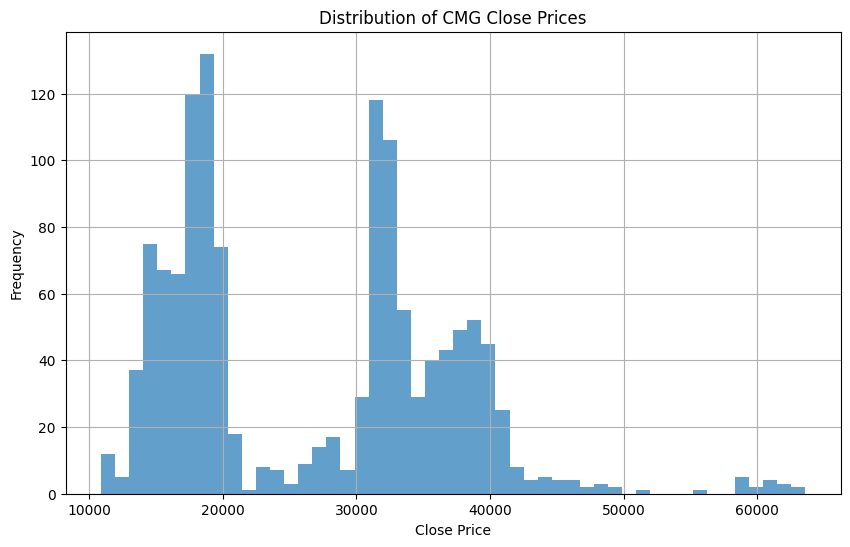
\includegraphics[width=1\textwidth]{bibliography/Figure/CMG_histogram.png}
        \caption{CMG stock price's histogram}
        \label{fig:2}
    \end{minipage}
\end{figure}
\section{Methodology}
\subsection{Linear Regression}
Simple Linear Regression estimates the relationship between a scalar response y and a single explanatory variable $x$ (also called dependent variable $x$ and independent variable $x$), given a set of data that includes observations for both of these variables for a particular sample. \cite{b5}

The basic model for multiple linear regression is:
\begin{equation}
    Y = \beta_0 + \beta_1X_1 + \beta_2X_2 + ... + \beta_mX_m + \mathcal{E}
\end{equation}

Where:
\begin{itemize}
    \item $Y$ is dependent variable;
    \item $X_1$, … $X_m$ is the distinct independent or predictor variables;
    \item $\beta_0$ is the $y$-intercept (value of $y$ when all other parameters are set to 0);
    \item $\beta_1$, ... $\beta_m$ is the regression coefficient of the independent variable;
    \item $\mathcal{E}$ is model error.
\end{itemize}


\subsection{ARIMA}
ARIMA is the abbreviation for “Autoregressive integrated moving average”. The ARIMA model is popularly used to forecast univariate time series data. ARIMA model can handle a time series if it is stationary and has no data missing \cite{b6}. This method is used in multiple studies for forecasting.

ARIMA models are expressed in the form of ARIMA (p,d,q) \cite{b7}. All p, d, and q are non-negative numbers.

\begin{enumerate}
    \item$AR$ is Auto Regression, and p is the number of autoregressive terms \cite{b8}. The equation for AR model is:
          \begin{equation}
              Y = \mu + \varphi_1Y_{t-1} + \varphi_2Y_{t-2} + ... + \varphi_pY_{t-p} + \varepsilon_t
          \end{equation}
          which:
          \begin{itemize}
              \item $Y$ is the current value;
              \item $\mu$ is the constant term;
              \item $p$ is the number of orders;
              \item $\varphi$ is the auto-regression coefficient and $\varepsilon_t$ is the error;
          \end{itemize}
    \item MA is the Moving Average, and q is the number of terms in the moving average [5]. The equation for MA model is:
          \begin{equation}
              Y = \mu + \theta_1Y_{t-1} + \theta_2Y_{t-2} + ... + \theta_pY_{t-p} + \varepsilon_t
          \end{equation}
          which:
          \begin{itemize}
            \item $Y_t$ is the current value;
            \item $\mu$ is the constant term;
            \item $p$ is the number of orders;
            \item $\theta$ is the moving average coefficient and $\varepsilon_t$ is the error
          \end{itemize}
    \item Last, the I part is Integrated, and d is the number of differences (order) required to make it a stationary sequence.
\end{enumerate}

After combining them, we will have the ARIMA(p, d, q) express as follow:
\begin{equation}
    \begin{aligned}
        \Delta Y_t = \mu + \varphi_1Y_{t-1} + \varphi_2Y_{t-2} + ... +\varphi_pY_{t-p} \\
        + \theta_1Y_{t-1} + \theta_2Y_{t-2} + ... + \theta_pY_{t-p} + \varepsilon_t
    \end{aligned}
\end{equation}

\subsection{Seasonal ARIMAX}
Seasonal ARIMAX (SARIMAX) is an advancement of the seasonal ARIMA with external feature variables (X) called SARIMAX ($p, d, q$) ($P,D,Q$)s ($X$) to improve its prediction and performance \cite{b9}. Where $X$ is the vector of external variables; where the small letter parentheses part ($p,d,q$) indicates the non-seasonal part of model while the capital letter part ($P,D,Q$)[$s$] indicates the seasonal part of model, $s$ being the number of periods per season \cite{b4}. The external variables can be modeled by multi linear regression equation is expressed as equation (1). The general seasonal autoregressive integrated moving average (SARIMA) model written as follows:
\begin{equation}
    \Phi_P(B^S)\phi_p(B)\bigtriangledown_S^D\bigtriangledown^d = \theta_q(B)\Theta_Q(B^S)\varepsilon_t
\end{equation}
where:
\begin{itemize}
    \item $\Phi_P(B^S) = (1 - \Phi_1B^S - ... - \Phi_pB^{sP})$ is the seasonal AR operator of order P
    \item $\phi_p(B) = (1 - \phi_1B - ... - \phi_pB^p)$ is the regular AR operator of order p;
    \item $\bigtriangledown_S^D = (1 - B)^d$ represents the seasonal differences and $\bigtriangledown_S^D = (1 - B^S)^D$ the regular differences;
    \item $\Theta_Q(B^S) = (1 - \Theta_1B^S - ... - \Theta_QB^{sQ})$ is the seasonal moving average operator of order Q;
    \item $\theta_q(B) = (1 - \theta_1B - ... - \theta_qB^q) $ is the regular moving average operator of order q;
    \item $\varepsilon_t$ is a white noise process.
\end{itemize}

SARIMAX model demonstrates the use of exogenous variables by using the concept of “regression with SARIMA errors”. In current study, the SARIMAX method was organized to forecast the stock price, the $X$ feature is the low price of the stock.The model can be written as:
\begin{equation}
    y_t = \beta x_t + z_t
\end{equation}

This equation is just a linear regression to depict the linear effect of exogenous variables on $y_t$. The error term $z_t$ follows the SARIMA process and can be described by usual SARIMA equation as
\begin{equation}
    \Phi_P(B^S)\phi_p(B)\bigtriangledown_S^D\bigtriangledown^dz_t = \theta_q(B)\Theta_Q(B^S)\varepsilon_t
\end{equation}

where all the notations and operators have same meaning as above \cite{b4}.
\subsection{Recurrent Neural Network}
Recurrent Neural Networks is a type of neural network that can be used to model sequence data. RNNs, which are formed from feedforward networks, are similar to human brains in their behaviour. Simply said, recurrent neural networks can anticipate sequential data in a way that other algorithms can’t \cite{b10}. RNN processes sequence data by connecting previous outputs to current calculations, unlike traditional neural networks. It memorizes past information, incorporating it into current outputs, allowing for processing sequences of any length.
\begin{figure} [H]
    \centering
    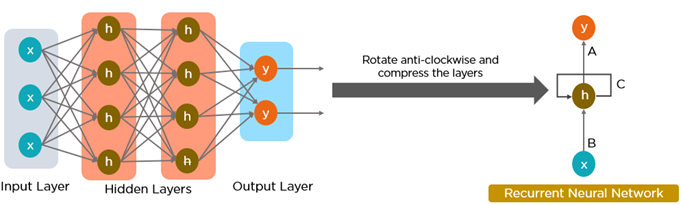
\includegraphics[width=0.5\textwidth]{bibliography/Figure/RNN_overview.png}
    \caption{Overview the Recurrent Neural Network}
    \label{fig:rnn-overview}
\end{figure}

The value $h$ of the hidden layer of RNN not only depends on the current input $x$, but also depends on the value $h$ of the last hidden layer, as shown in figure 8:
\begin{figure} [H]
    \centering
    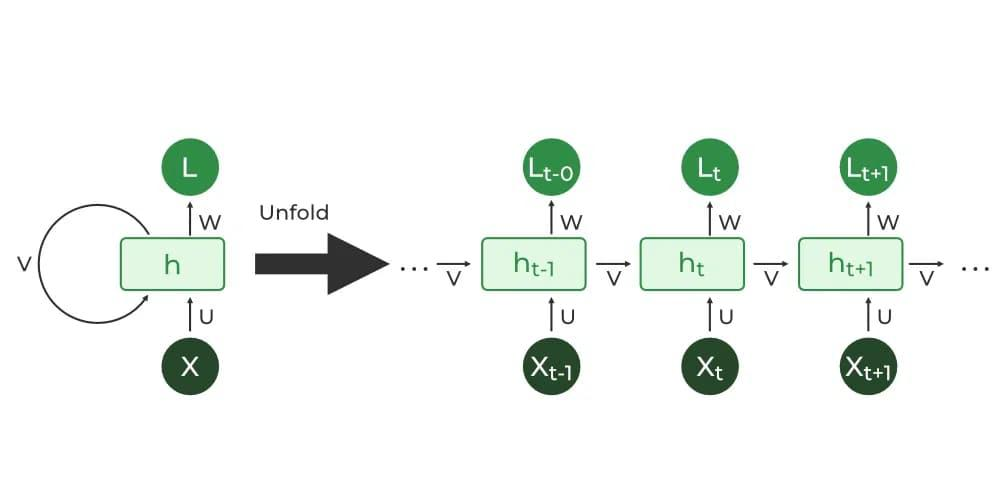
\includegraphics[width=0.5\textwidth]{bibliography/Figure/What-is-Recurrent-Neural-Network.jpg}
    \caption{RNN hidden layer calculate process.}
    \label{fig:rnn-hidden-layer}
\end{figure}
Among them, $t$ is the time, $x$ is the input layer, $h$ is the hidden layer, $L$ is the output layer, and the matrix $W$ is the last value of the hidden layer as the weight of this input. RNN training also uses the BP error back propagation algorithm, but there is a little difference. In the training process, the parameters $W, U, V$ are shared, but the traditional fully connected neural network is not. And in using the gradient descent algorithm, the output of each step not only depends on the current step of the network, but also depends on the state of the previous steps of the network.

\subsection{Long Short-Term Memory}
Long short term memory (LSTM) \cite{b12} is a deformation structure of RNN by adding memory cell into hidden layer, so as to control the memory information of the time series data. Information is transmitted among different cells of hidden layer through several controllable gates (forget gate, input gate, output gate) \cite{b13}, thus the memory and forgetting extent of the previous and current information can be controlled. Compared with traditional RNN, the LSTM has the long term memory function and its gradient disappearance problem can be avoided. Two gates of LSTM are designed for controlling the state of memory cell, one is forget gate which indicates how much ‘‘memory’’ of the last moment’s cell can be saved, the other is input gate, which determines how much input of the current moment can be saved to the cell state, and controls the proportion of fusion of ‘‘historical’’ information and ‘‘current’’ stimulus. Finally, the output gate of LSTM is designed for controlling how much information is output for cell status.
\begin{figure} [H]
    \centering
    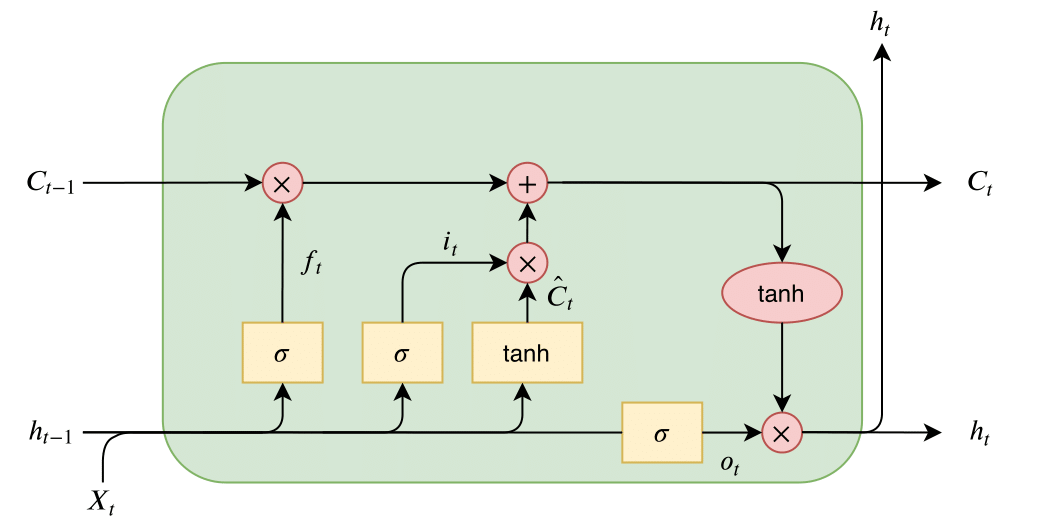
\includegraphics[width=0.5\textwidth]{bibliography/Figure/LSTM _structure.png}
    \caption{LSTM Structure network}
    \label{fig:LSTM structure}
\end{figure}

In Figure 9, $\sigma$ is the sigmoid function shown in equation (13), whose output is a value between 0 and 1. Here, 0 means ‘‘let nothing pass’’ while 1 means "let everything pass". Then the hyperbolic tangent function illustrated in Equation (14), is used to overcome the problem of gradient disappearance.
\begin{equation}
    f_t = \sigma(W_f.[h_{t-1}, X_t] + b_f)
\end{equation}
\begin{equation}
    i_t = \sigma(W_i.[h_{t-1}, X_t] + b_i)
\end{equation}
\begin{equation}
    \hat{C}_t = tanh(W_c.[h_{t-1}, X_t] + b_c)
\end{equation}
\begin{equation}
    C_t = f_t*C_{t-1} + i_t + \hat{C}_t
\end{equation}
\begin{equation}
    O_t = \sigma(W_o.[h_{t-1}, X_t] + b_o)
\end{equation}
\begin{equation}
    sigmoid(x) = \frac{1}{1+e^{-x}}
\end{equation}
\begin{equation}
    tanh(x) = \frac{e^x - e^{-x}}{e^x + e^{-x}}
\end{equation}

where:
\begin{itemize}
    \item $W_f, W_i, W_c$ and $W_o$ are input weights
    \item $b_f, b_i, b_c$ and $b_o$ are bias weights
    \item $t$ represents the current time state
    \item $t - 1$ is the previous time state
    \item $X$ represents input
    \item $H$ represents output
    \item $C$ is the cell status
\end{itemize}
\subsection{Gate Recurrent Unit}
GRU is one of the most popular improved variants of RNN with a special gated recurrent neural network based on optimized LSTM. The GRU internal structure is similar to the internal structure of the LSTM, except that the GRU associates the input gate and the forget gate in the LSTM unit into a single update gate. This model has two gates: one is the update gate, which controls the extent and retains previous information in the current state; the other represents the reset gate which determines whether the previous information and the current state are to be associated \cite{b14}. Figure 10 shows the basic design of a GRU unit.
\begin{figure} [H]
    \centering
    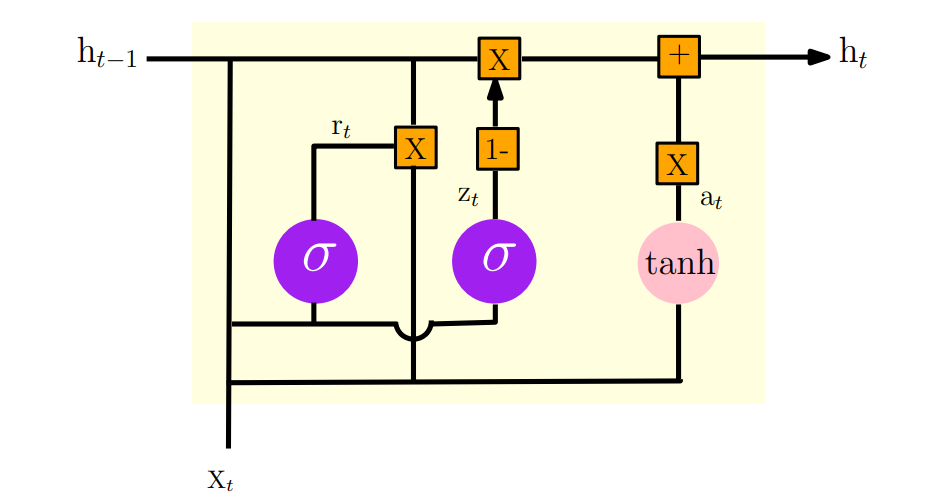
\includegraphics[width=0.5\textwidth]{bibliography/Figure/GRU.png}
    \caption{The structure of GRU units}
    \label{fig:GRU structure}
\end{figure}
According to Figure 10, the formulas of GRU can be given as:
\begin{equation}
    z_t = \sigma(w_z[h_{t - 1}, X_t] + b_z)
\end{equation}
\begin{equation}
    r_t = \sigma(w_r[h_{t - 1}, X_t] + b_r)
\end{equation}
\begin{equation}
    a_t = tanh(r_t * w_a[h_{t - 1}, X_t] + b_a)
\end{equation}
\begin{equation}
    h_t = (1 - z_t) * a_t + z_t * h_{t - 1}
\end{equation}
where:
\begin{itemize}
    \item $X_t$ is the vector input of training data at time $t$.
    \item $h_t$ is the outcome of the current layer at time $t$.
    \item $z_t$ and $r_t$ represent the update and the reset gates respectively.
    \item $t$ is the candidate activation.
\end{itemize}
\subsection{Gradient Boosting Regressor}

Gradient Boosting Regressor (GBR) is a powerful ensemble learning technique that constructs predictive models in a stage-wise fashion by combining multiple weak learners, typically decision trees, to enhance predictive accuracy. GBR is particularly effective for time-series forecasting due to its ability to capture temporal dependencies and trends in the data.

The whole process of building a GBR model includes:
\subsubsection{Initial Model}

GBR commences with an initial constant model:
\begin{equation}
    \hat{F}_0(x) = \arg\min_{c} \sum_{i=1}^{N} L(y_i, c),
\end{equation}
where:
\begin{itemize}
    \item \(\hat{F}_0(x)\) represents the initial prediction model,
    \item \(L(y_i, c)\) denotes the loss function,
    \item \(y_i\) signifies the actual values, and
    \item \(c\) stands for a constant.
\end{itemize}

\subsubsection{Pseudo-Residuals}

At each stage \(m\), the model computes pseudo-residuals to identify the errors of the current model:
\begin{equation}
    r_{im} = -\left[\frac{\partial L(y_i, \hat{F}(x_i))}{\partial \hat{F}(x_i)}\right]_{\hat{F}(x) = \hat{F}_{m-1}(x)},
\end{equation}
where:
\begin{itemize}
    \item \(r_{im}\) refers to the pseudo-residuals,
    \item \(L\) stands for the loss function, and
    \item \(\hat{F}(x_i)\) represents the current model prediction.
\end{itemize}

\subsubsection{Model Update}

A new decision tree \(h_m(x)\) is fitted to the pseudo-residuals, and the model is updated:
\begin{equation}
    \hat{F}_m(x) = \hat{F}_{m-1}(x) + \nu h_m(x),
\end{equation}
where:
\begin{itemize}
    \item \(\hat{F}_m(x)\) denotes the updated model,
    \item \(\nu\) represents the learning rate, and
    \item \(h_m(x)\) stands for the new tree.
\end{itemize}
\subsubsection{Application in Time-Series Forecasting}
\begin{algorithm}[H]
    \caption{Gradient Boosting Regressor for Time-Series Forecasting}
    \label{alg:gbr-time-series}
    
    \textbf{Input:} Time-series data \( \{y_1, y_2, \ldots, y_T\} \), Window size \( n \), Iterations \( M \), Learning rate \( \nu \)
    
    \textbf{Output:} Forecasted values \( \{\hat{y}_{T+1}, \hat{y}_{T+2}, \ldots, \hat{y}_{T+h}\} \) for \( h \) steps ahead
    
    \textbf{Initialization:} Initialize \( \hat{F}_0(x) \) using the initial model:
    \[
    \hat{F}_0(x) = \arg\min_{c} \sum_{i=1}^{n} L(y_i, c)
    \]
    Set \( \hat{F}(x) = \hat{F}_0(x) \)
    
    \textbf{Training and Forecasting:}
    \begin{enumerate}
        \item Initialize \( t = n+1 \)
        \item \textbf{While} \( t \leq T+h \):
        \begin{enumerate}
            \item \textbf{Construct the feature vector:}
            \[ 
                X_t = [y_{t-1}, y_{t-2}, \ldots, y_{t-n}] 
            \]
            \item \textbf{Compute pseudo-residuals:}
                \[
                r_{it} = -\frac{\partial L(y_i, \hat{F}(X_i))}{\partial \hat{F}(X_i)} \bigg|_{\hat{F}(X_i) = \hat{F}(X_i)}
                \]
            \item \textbf{Train weak learner:}
                \[
                \begin{aligned}
                \text{weak learner} &= \arg\min_{h} \sum_{i=1}^{t-1} \left[ r_{it} - h(X_i) \right]^2
                \end{aligned}
                \]
            \item \textbf{Update the model:}
                \[
                \hat{F}(x) \leftarrow \hat{F}(x) + \nu \cdot \text{weak learner}(x)
                \]
            \item \textbf{Forecast:}
                \[
                \hat{y}_{t} = \hat{F}(X_t)
                \]
            \item \textbf{Slide window forward \( t \):} \( t = t + 1 \)
        \end{enumerate}
    \end{enumerate}
\end{algorithm}

\subsection{Decomposition Linear}
Decomposition Linear or DLinear, is a model introduced for time series forecasting.  It first decomposes a raw data input into a trend component by a moving average kernel and a remainder (seasonal) component. Then, two
one-layer linear layers are applied to each component,
and we sum up the two features to get the final prediction. By explicitly handling trend, DLinear enhances
the performance of a vanilla linear when there is a clear
trend in the data \cite{b15}.

\begin{figure} [H]
    \centering
    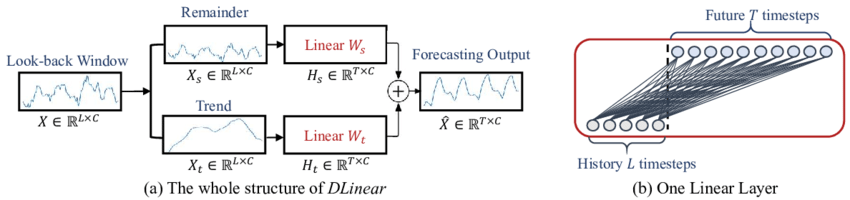
\includegraphics[width=0.5\textwidth]{bibliography/Figure/Illu_DLinear.png}
    \caption{Illustration of the Decomposition Linear Model}
    \label{fig:DLinear Illustration}
\end{figure}

The overall structure of DLinear is shown in Figure 11(a). The whole process is:

\subsubsection{Decomposition}
DLinear decomposes the time series $\mathbf{x} \in \mathbb{R}^{L \times C}$ into trend and seasonal components:

\begin{equation}
    \mathbf{x}(t) = \mathbf{T}(t) + \mathbf{S}(t) + \epsilon(t),
\end{equation}

where:
\begin{itemize}
    \item $\mathbf{T}(t)$ represents the trend component,
    \item $\mathbf{S}(t)$ represents the seasonal component,
    \item $\epsilon(t)$ is the residual (noise) component.
\end{itemize}

\subsubsection{Trend Extraction}
The trend component $\mathbf{T}(t)$ captures the long-term progression of the time series. It can be extracted using methods such as moving averages or polynomial fitting:

\begin{equation}
    \mathbf{T}(t) = \frac{1}{2k+1} \sum_{i=-k}^{k} \mathbf{x}(t+i),
\end{equation}

where $k$ is the window size for the moving average.

\subsubsection{Seasonal Component}
The seasonal component $\mathbf{S}(t)$ captures the repeating patterns within the time series. It can be obtained by removing the trend from the original series:
\begin{equation}
    \mathbf{S}(t) = \mathbf{x}(t) - \mathbf{T}(t).
\end{equation}

\subsubsection{Linear Modeling}
Separate linear models are used to predict the trend and seasonal components:
\begin{align}
    \hat{\mathbf{T}}(t+h) & = \mathbf{W}_T \mathbf{T}(t) + \mathbf{b}_T \\
    \hat{\mathbf{S}}(t+h) & = \mathbf{W}_S \mathbf{S}(t) + \mathbf{b}_S
\end{align}

where:
\begin{itemize}
    \item $\mathbf{W}_T$ and $\mathbf{W}_S$ are weight matrices for the trend and seasonal components, respectively,
    \item $\mathbf{b}_T$ and $\mathbf{b}_S$ are bias vectors for the trend and seasonal components, respectively,
    \item $t+h$ indicates the forecasted value $h$ steps ahead from the current time $t$, as illustrated in Figure 11(b).
\end{itemize}

The final forecast \( \hat{\mathbf{x}}(t+h) \) is obtained by combining the predictions from the trend and seasonal models:
\begin{equation}
    \hat{\mathbf{x}}(t+h) = \hat{\mathbf{T}}(t+h) + \hat{\mathbf{S}}(t+h).
\end{equation}
DLinear offers an efficient and effective approach to time series forecasting by leveraging decomposition and linear transformations. This model addresses the limitations of traditional Transformers, making it suitable for long-term forecasting tasks.
\section{RESULT}
In this section, we will evaluate eight different models in forecasting: Linear Regression, ARIMA, SARIMAX, LSTM, GRU, DLinear, RNN, and Gradient Boosting Regressor. Initially, we will preprocess the original time series dataset. Following preprocessing, we will divide the data into train and test sets using three different ratios: 70:30, 80:20 and 90:10. Each model will be trained on the training set and subsequently used to make predictions on the test set. The performance of these models will be assessed using the following evaluation metrics: Mean Squared Error (MSE), Mean Absolute Error (MAE), and Root Mean Squared Error (RMSE). The results are presented in the tables below.
\subsection{CMG}
\begin{table}[H]
    \renewcommand{\arraystretch}{1.5}
    \centering
    \begin{tabular}{|c|c|p{1cm}|p{1cm}|p{1cm}|}
        \hline
        \textbf{Model} & \textbf{Train/Test} & \textbf{RMSE} & \textbf{MAE} & \textbf{MAPE} \\
        \hline
        % Linear Regression
        \multirow{3}{*}{LR}
                       & 7 - 3               & 4776.167      & 3242.941     & 8.655\%       \\
        \cline{2-5}
                       & 8 - 2               & 5613.133      & 2972.978     & 6.365\%       \\
        \cline{2-5}
                       & 9 - 1               & 7630.459      & 4249.712     & 8.081\%       \\
        \hline
        % ARIMA
        \multirow{3}{*}{ARIMA}
                       & 7 - 3               & 5590.559      & 3396.414     & 8.036\%       \\
        \cline{2-5}
                       & 8 - 2               & 7949.917      & 5917.192     & 13.443\%      \\
        \cline{2-5}
                       & 9 - 1               & 8392.384      & 5363.964     & 10.641\%      \\
        \hline
        % SARIMAX
        \multirow{3}{*}{SARIMAX}
                       & 7 - 3               & 4790.479      & 3368.235     & 8.027\%       \\
        \cline{2-5}
                       & 8 - 2               & 1606.532      & 1266.783     & 2.998\%       \\
        \cline{2-5}
                       & 9 - 1               & 1880.078      & 1333.986     & 2.803\%       \\
        \hline
        % RNN
        \multirow{3}{*}{RNN}
                       & 7 - 3               & 1310.051      & 803.027      & 2.022\%       \\
        \cline{2-5}
                       & 8 - 2               & 1434.569      & 973.583      & 2.283\%       \\
        \cline{2-5}
                       & 9 - 1               & 1899.021      & 1241.602     & 2.615\%       \\
        \hline
        % GRU
        \multirow{3}{*}{GRU}
                       & 7 - 3               & 1256.333      & 800.386      & 2.037\%       \\
        \cline{2-5}
                       & 8 - 2               & 1636.782      & 1039.329     & 2.393\%       \\
        \cline{2-5}
                       & 9 - 1               & 1901.258      & 1256.691     & 2.654\%       \\
        \hline
        % LSTM
        \multirow{3}{*}{LSTM}
                       & 7 - 3               & 1455.690      & 834.627      & 2.051\%       \\
        \cline{2-5}
                       & 8 - 2               & 1687.759      & 1013.020     & 2.287\%       \\
        \cline{2-5}
                       & 9 - 1               & 1975.455      & 1264.345     & 2.642\%       \\
        \hline
        % GBR
        \multirow{3}{*}{GBR}
                       & 7 - 3               & 4805.334      & 1856.740     & 3.867\%       \\
        \cline{2-5}
                       & 8 - 2               & 5885.479      & 2586.670     & 5.133\%       \\
        \cline{2-5}
                       & 9 - 1               & 8742.394      & 5095.510     & 9.776\%       \\
        \hline
        % DLinear
        \multirow{3}{*}{DLinear}
                       & 7 - 3               & 941.648       & 610.784      & 1.590\%       \\
        \cline{2-5}
                       & 8 - 2               & 995.657       & 620.887      & 1.442\%       \\
        \cline{2-5}
                       & 9 - 1               & 1294.638      & 911.389      & 1.972\%       \\
        \hline
    \end{tabular}
    \caption{Performance Metrics on CMG's test set}
    \label{tab:performance_metrics_cmg}
\end{table}
\subsection{FPT}
\begin{table}[H]
    \renewcommand{\arraystretch}{1.5}
    \centering
    \begin{tabular}{|c|c|p{1.2cm}|p{1.2cm}|p{1cm}|}
        \hline
        \textbf{Model} & \textbf{Train/Test} & \textbf{RMSE} & \textbf{MAE} & \textbf{MAPE} \\
        \hline
        % Linear Regression
        \multirow{3}{*}{LR}
                       & 7 - 3               & 13208.213     & 11051.009    & 13.721\%      \\
        \cline{2-5}
                       & 8 - 2               & 15941.794     & 12193.876    & 11.668\%      \\
        \cline{2-5}
                       & 9 - 1               & 20588.570     & 16918.134    & 14.564\%      \\
        \hline
        % ARIMA
        \multirow{3}{*}{ARIMA}
                       & 7 - 3               & 19697.622     & 13787.839    & 13.429\%      \\
        \cline{2-5}
                       & 8 - 2               & 25634.306     & 21517.835    & 20.593\%      \\
        \cline{2-5}
                       & 9 - 1               & 16524.874     & 11914.706    & 9.908\%       \\
        \hline
        % SARIMAX
        \multirow{3}{*}{SARIMAX}
                       & 7 - 3               & 13980.543     & 10637.005    & 10.691\%      \\
        \cline{2-5}
                       & 8 - 2               & 2689.828      & 2194.418     & 2.135\%       \\
        \cline{2-5}
                       & 9 - 1               & 11337.132     & 8609.467     & 7.251\%       \\
        \hline
        % RNN
        \multirow{3}{*}{RNN}
                       & 7 - 3               & 2279.840      & 1514.533     & 1.633\%       \\
        \cline{2-5}
                       & 8 - 2               & 2917.896      & 1973.960     & 1.890\%       \\
        \cline{2-5}
                       & 9 - 1               & 3103.424      & 2241.372     & 1.969\%       \\
        \hline
        % GRU
        \multirow{3}{*}{GRU}
                       & 7 - 3               & 2130.231      & 1433.697     & 1.563\%       \\
        \cline{2-5}
                       & 8 - 2               & 2809.575      & 2001.863     & 1.955\%       \\
        \cline{2-5}
                       & 9 - 1               & 2672.474      & 1886.464     & 1.658\%       \\
        \hline
        % LSTM
        \multirow{3}{*}{LSTM}
                       & 7 - 3               & 3157.352      & 2151.767     & 2.231\%       \\
        \cline{2-5}
                       & 8 - 2               & 3512.565      & 2483.480     & 2.357\%       \\
        \cline{2-5}
                       & 9 - 1               & 2681.850      & 1870.596     & 1.642\%       \\
        \hline
        % GBR
        \multirow{3}{*}{GBR}
                       & 7 - 3               & 22226.841     & 14757.446    & 13.947\%      \\
        \cline{2-5}
                       & 8 - 2               & 27359.470     & 22065.749    & 20.665\%      \\
        \cline{2-5}
                       & 9 - 1               & 18090.845     & 13052.712    & 10.774\%      \\
        \hline
        % DLinear
        \multirow{3}{*}{DLinear}
                       & 7 - 3               & 1521.300      & 1050.039     & 1.185\%       \\
        \cline{2-5}
                       & 8 - 2               & 1563.924      & 1083.996     & 1.094\%       \\
        \cline{2-5}
                       & 9 - 1               & 1826.883      & 1288.223     & 1.161\%       \\
        \hline
    \end{tabular}
    \caption{Performance Metrics on FPT's test set}
    \label{tab:performance_metrics_fpt}
\end{table}
\subsection{ITD}
\begin{table}[H]
    \renewcommand{\arraystretch}{1.5}
    \centering
    \begin{tabular}{|c|c|p{1cm}|p{1cm}|p{1cm}|}
        \hline
        \textbf{Model} & \textbf{Train/Test} & \textbf{RMSE} & \textbf{MAE} & \textbf{MAPE} \\
        \hline
        % Linear Regression
        \multirow{3}{*}{LR}
                       & 7 - 3               & 5049.939      & 4772.159     & 45.394\%      \\
        \cline{2-5}
                       & 8 - 2               & 4119.015      & 3919.348     & 38.153\%      \\
        \cline{2-5}
                       & 9 - 1               & 3584.478      & 3542.331     & 35.514\%      \\
        \hline
        % ARIMA
        \multirow{3}{*}{ARIMA}
                       & 7 - 3               & 1205.208      & 1073.681     & 9.719\%       \\
        \cline{2-5}
                       & 8 - 2               & 2181.237      & 1900.551     & 18.846\%      \\
        \cline{2-5}
                       & 9 - 1               & 595.809       & 380.715      & 3.592\%       \\
        \hline
        % SARIMAX
        \multirow{3}{*}{SARIMAX}
                       & 7 - 3               & 187.480       & 153.968      & 1.417\%       \\
        \cline{2-5}
                       & 8 - 2               & 148.763       & 115.969      & 1.094\%       \\
        \cline{2-5}
                       & 9 - 1               & 150.452       & 121.827      & 1.201\%       \\
        \hline
        % RNN
        \multirow{3}{*}{RNN}
                       & 7 - 3               & 321.746       & 223.305      & 2.045\%       \\
        \cline{2-5}
                       & 8 - 2               & 272.520       & 191.926      & 1.823\%       \\
        \cline{2-5}
                       & 9 - 1               & 285.653       & 210.604      & 2.037\%       \\
        \hline
        % GRU
        \multirow{3}{*}{GRU}
                       & 7 - 3               & 308.320       & 212.661      & 1.948\%       \\
        \cline{2-5}
                       & 8 - 2               & 287.198       & 216.931      & 2.064\%       \\
        \cline{2-5}
                       & 9 - 1               & 287.089       & 187.537      & 1.791\%       \\
        \hline
        % LSTM
        \multirow{3}{*}{LSTM}
                       & 7 - 3               & 313.356       & 215.751      & 1.972\%       \\
        \cline{2-5}
                       & 8 - 2               & 269.044       & 190.121      & 1.803\%       \\
        \cline{2-5}
                       & 9 - 1               & 278.773       & 186.645      & 1.786\%       \\
        \hline
        % GBR
        \multirow{3}{*}{GBR}
                       & 7 - 3               & 287.311       & 224.065      & 2.053\%       \\
        \cline{2-5}
                       & 8 - 2               & 239.767       & 182.027      & 1.735\%       \\
        \cline{2-5}
                       & 9 - 1               & 267.945       & 209.760      & 2.055\%       \\
        \hline
        % DLinear
        \multirow{3}{*}{DLinear}
                       & 7 - 3               & 253.810       & 185.018      & 1.700\%       \\
        \cline{2-5}
                       & 8 - 2               & 250.853       & 198.298      & 1.875\%       \\
        \cline{2-5}
                       & 9 - 1               & 286.739       & 227.045      & 2.211\%       \\
        \hline
    \end{tabular}
    \caption{Performance Metrics on ITD's test set}
    \label{tab:performance_metrics_itd}
\end{table}
\subsection{Forecasting Plot}
\begin{figure} [H]
    \centering
    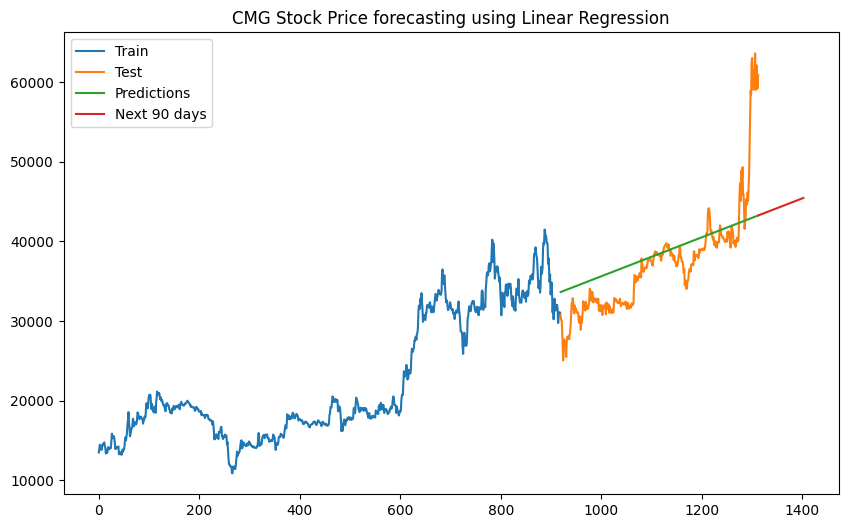
\includegraphics[width=0.4\textwidth]{bibliography/Figure/LR_CMG_73.png}
    \caption{Linear Regression - CMG - 73}
    \label{fig:LR_CMG_73}
\end{figure}
\begin{figure} [H]
    \centering
    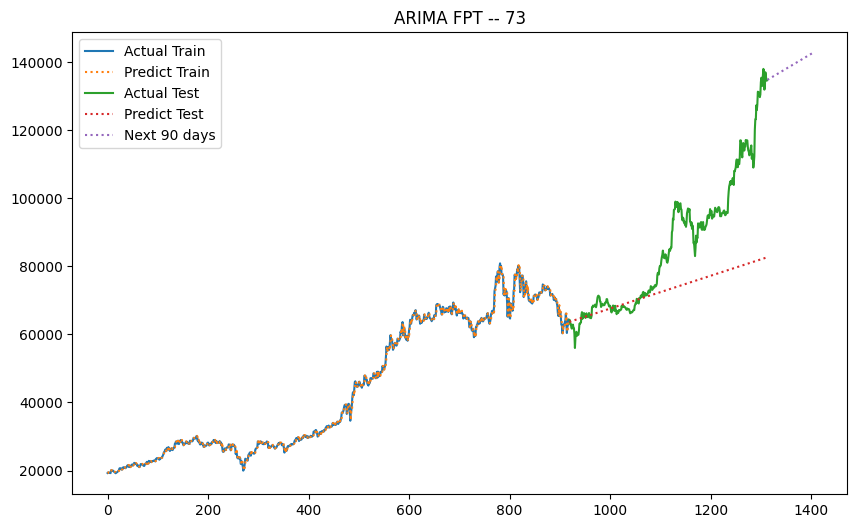
\includegraphics[width=0.4\textwidth]{bibliography/Figure/ARIMA_FPT_73.png}
    \caption{ARIMA - FPT - 73}
    \label{fig:ARIMA_FPT_73}
\end{figure}
\begin{figure} [H]
    \centering
    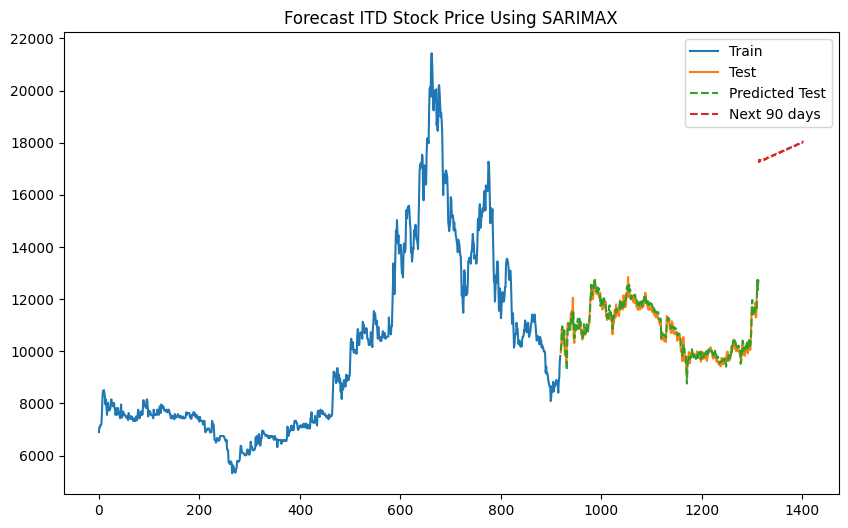
\includegraphics[width=0.4\textwidth]{bibliography/Figure/SARIMAX_ITD_73.png}
    \caption{SARIMAX - ITD - 73}
    \label{fig:SARIMAX_ITD_73}
\end{figure}
\begin{figure} [H]
    \centering
    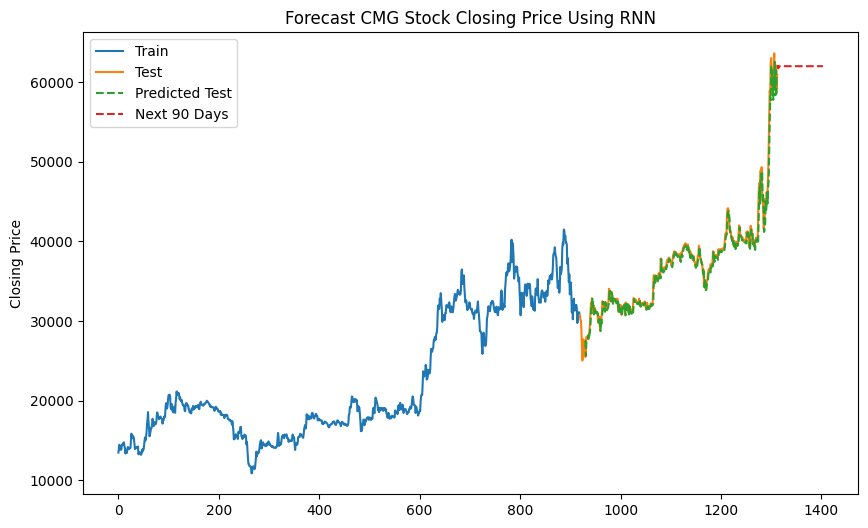
\includegraphics[width=0.4\textwidth]{bibliography/Figure/RNN_CMG_73.png}
    \caption{RNN - CMG - 73}
    \label{fig:RNN_CMG_73}
\end{figure}
\begin{figure} [H]
    \centering
    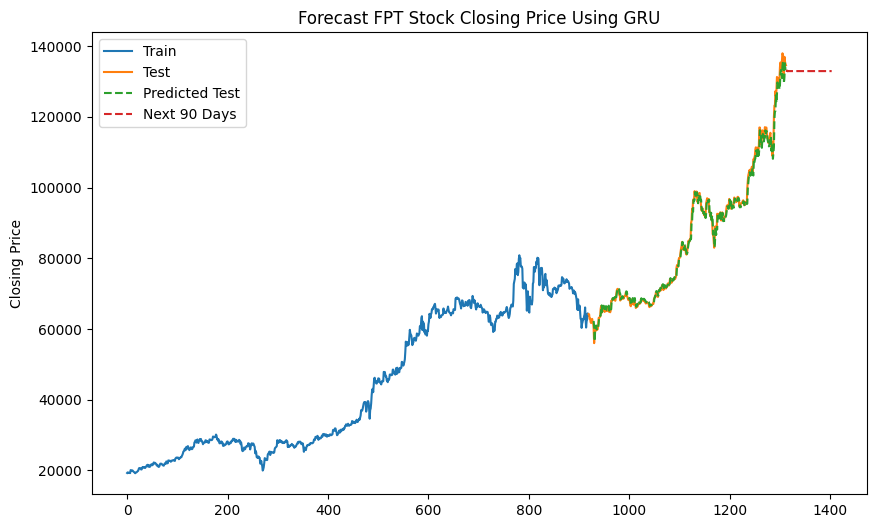
\includegraphics[width=0.4\textwidth]{bibliography/Figure/GRU_FPT_73.png}
    \caption{GRU - FPT - 73}
    \label{fig:GRU_FPT_73}
\end{figure}
\begin{figure} [H]
    \centering
    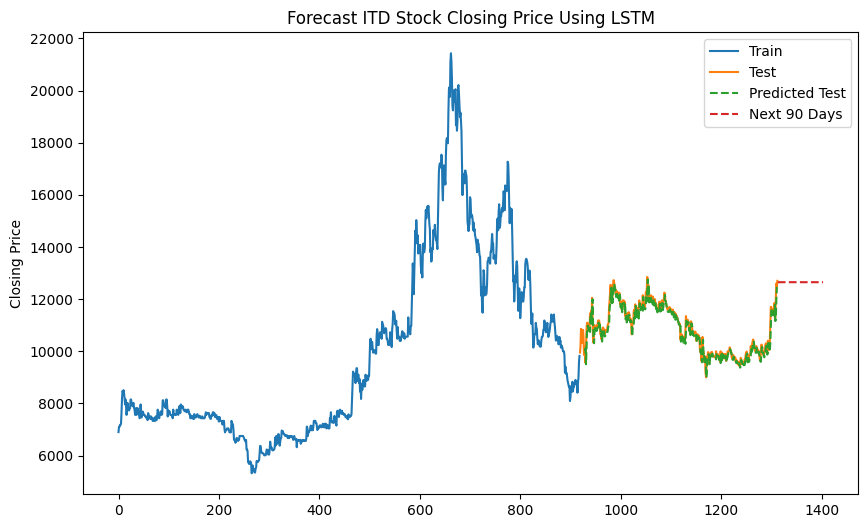
\includegraphics[width=0.4\textwidth]{bibliography/Figure/LSTM_ITD_73.png}
    \caption{LSTM - ITD - 73}
    \label{fig:LSTM_ITD_73}
\end{figure}
\begin{figure} [H]
    \centering
    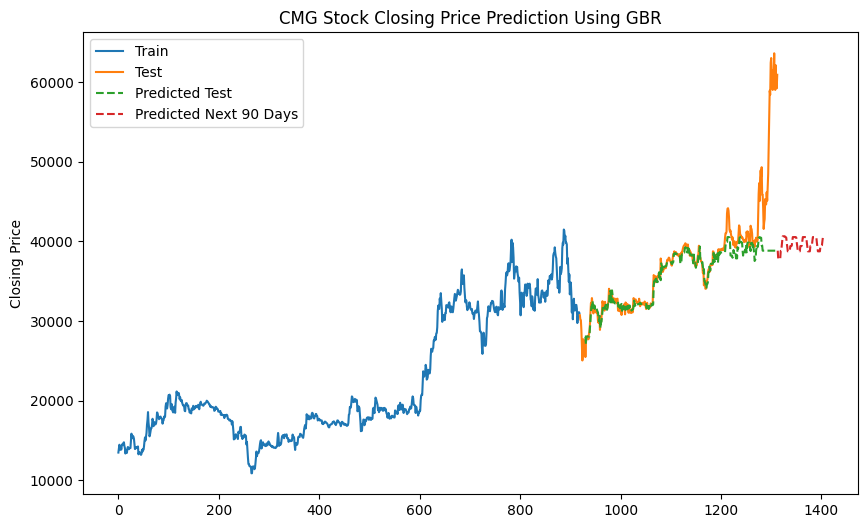
\includegraphics[width=0.4\textwidth]{bibliography/Figure/GBR_CMG_73.png}
    \caption{GBR - CMG - 73}
    \label{fig:GBR_CMG_73}
\end{figure}
\begin{figure} [H]
    \centering
    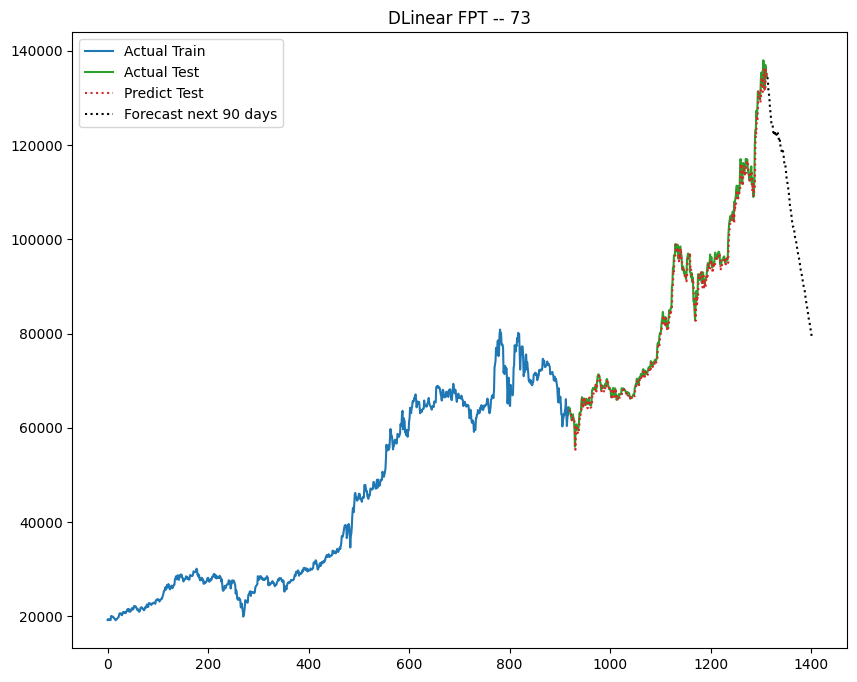
\includegraphics[width=0.4\textwidth]{bibliography/Figure/DLinear_FPT_73.png}
    \caption{DLinear - FPT - 73}
    \label{fig:DLinear_FPT_73}
\end{figure}

\section{Conclusion}
In this study, we forecasted the stock prices of three Vietnamese tech companies: CMG, FPT, and ITD. We evaluated eight different models using three train-test splits (70:30, 80:20, 90:10). For CMG and FPT stocks, the DLinear model consistently delivered the lowest RMSE, MAE, and MAPE across all splits, making it the most effective model for these stocks. In contrast, the SARIMAX model proved to be the best for ITD stock, achieving the lowest error metrics in all splits.

The stock forecasts for CMG and FPT show that the DLinear model effectively captures stable trends, offering reliable insights for investors. For ITD, the SARIMAX model's success highlights the importance of considering specific temporal dynamics and exogenous factors.

Leveraging these findings, stakeholders can better understand the stock performance of these Vietnamese tech companies and make informed investment decisions. Our continued efforts will aim to provide even more accurate forecasts to support market analyses and growth in the tech sector.

Future research will focus on developing more sophisticated models to enhance prediction accuracy and robustness. Our goal is to refine these models further and explore new techniques to achieve higher precision in stock price forecasting.
\section*{Acknowledgments}
We would like to express our deepest gratitude to \textbf{Assoc. Prof. Dr. Nguyen Dinh Thuan} and \textbf{Mr. Nguyen Minh Nhut} for their unwavering care, support, and invaluable guidance throughout this course. Your expertise and enthusiasm have greatly enriched our knowledge and played a crucial role in the successful completion of this project.

This report would not have been possible without your assistance and tireless efforts in guiding us. Thank you for inspiring us to keep moving forward and achieve our goals.
%% UNCOMMENT these lines below (and remove the 2 commands above) if you want to embed the bibliografy.
\begin{thebibliography}{00}
    \bibitem{b1} Pai, P.-F. and Lin, C.H. (2005) ‘A hybrid ARIMA and support vector machines model in stock price forecasting’.
    \bibitem{b2} Vijh, M. et al. (2020) ‘Stock Closing Price Prediction using Machine Learning Techniques’.
    \bibitem{b3}Nelson, D.M., Pereira, A.C.M. and Oliveira, R.A. de (2017) ‘Stock market’s price movement prediction with LSTM neural networks’.
    \bibitem{b4}S. Kumar, A. Gupta, K. Arora, and K. Vatta, “Effect of Rainfall in Predicting Tomato Prices in India: An Application of SARIMAX and NARX Model,” vol. 32, pp. 159–164, Dec. 2022.
    \bibitem{b5}M. Tranmer, J. Murphy, M. Elliot, and M. Pampaka, “Multiple Linear Regression (2nd Edition)”.
    \bibitem{b6}V. Ş. Ediger and S. Akar, “ARIMA forecasting of primary energy demand by fuel in Turkey,” Energy Policy, vol. 35, no. 3, pp. 1701–1708, Mar. 2007.
    \bibitem{b7}B. Dey, B. Roy, S. Datta, and T. S. Ustun, “Forecasting ethanol demand in India to meet future blending targets: A comparison of ARIMA and various regression models,” Energy Rep., vol. 9, pp. 411–418, Mar. 2023.
    \bibitem{b8}X. Jin and C. Yi, “The Comparison of Stock Price Prediction Based on Linear Regression Model and Machine Learning Scenarios,” presented at the 2022 International Conference on Bigdata Blockchain and Economy Management (ICBBEM 2022), Atlantis Press, Dec. 2022, pp. 837–842.
    \bibitem{b9}Manigandan P, Alam MS, Alharthi M, Khan U, Alagirisamy K, Pachiyappan D, Rehman A. Forecasting Natural Gas Production and Consumption in United States-Evidence from SARIMA and SARIMAX Models. Energies. 2021; 14(19):6021.
    \bibitem{b10}D. Kalita, “A Brief Overview of Recurrent Neural Networks (RNN),”Analytics Vidhya, Mar. 11, 2022.
    \bibitem{b11}U. Singh, M. Rizwan, M. Alaraj, and I. Alsaidan, “A Machine Learning-Based Gradient Boosting Regression Approach for Wind Power Production Forecasting: A Step towards Smart Grid Environments,” Aug. 2021.
    ‌\bibitem{b12} S. Hochreiter and J. Schmidhuber, ‘‘Long short-time memory,’’ Neural Comput., vol. 9, no. 8, pp. 1735–1780, 1997.
    \bibitem{b13}F. A. Gers, J. Schmidhuber, and F. Cummins, ‘‘Learning to forget:
    Continual prediction with LSTM,’’ Neural Comput., vol. 12, no. 10, pp. 2451–2471, Oct. 2000.
    \bibitem{b14}Mahjoub, S., Chrifi-Alaoui, L., Marhic, B., \& Delahoche, L. (2022). Predicting energy consumption using LSTM, multi-layer GRU and drop-GRU neural networks. Sensors, 22(11), 4062.
    \bibitem{b15}Zhou, T., Ma, Z., Zhou, Z., Chen, J., Wang, X., Jiang, Z., \& Jin, X. (2022).
    ‘‘Are Transformers Effective for Time Series Forecasting?’’. arXiv:2205.13504v3 [cs.AI] 17 Aug 2022.

\end{thebibliography}
%%%%%%%%%%%%%%%
\EOD

\end{document}